


\tikzset{every picture/.style={line width=0.75pt}} %set default line width to 0.75pt        

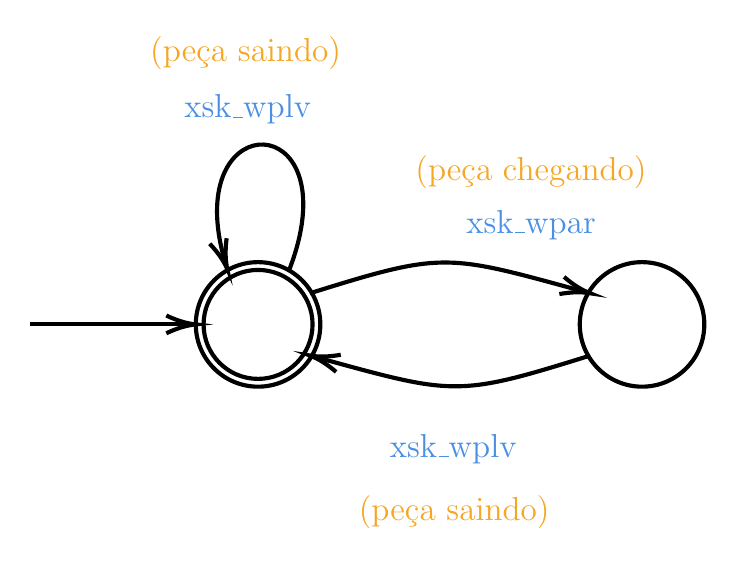
\begin{tikzpicture}[x=0.75pt,y=0.75pt,yscale=-1,xscale=1]
%uncomment if require: \path (0,1950); %set diagram left start at 0, and has height of 1950

%Shape: Circle [id:dp022173602878892806] 
\draw  [line width=1.5]  (190,1647) .. controls (190,1630.43) and (203.43,1617) .. (220,1617) .. controls (236.57,1617) and (250,1630.43) .. (250,1647) .. controls (250,1663.57) and (236.57,1677) .. (220,1677) .. controls (203.43,1677) and (190,1663.57) .. (190,1647) -- cycle ;
%Shape: Circle [id:dp423715485375872] 
\draw  [line width=1.5]  (193.75,1647) .. controls (193.75,1632.5) and (205.5,1620.75) .. (220,1620.75) .. controls (234.5,1620.75) and (246.25,1632.5) .. (246.25,1647) .. controls (246.25,1661.5) and (234.5,1673.25) .. (220,1673.25) .. controls (205.5,1673.25) and (193.75,1661.5) .. (193.75,1647) -- cycle ;
%Straight Lines [id:da5144723553129629] 
\draw [line width=1.5]    (110,1647) -- (187,1647) ;
\draw [shift={(190,1647)}, rotate = 180] [color={rgb, 255:red, 0; green, 0; blue, 0 }  ][line width=1.5]    (14.21,-4.28) .. controls (9.04,-1.82) and (4.3,-0.39) .. (0,0) .. controls (4.3,0.39) and (9.04,1.82) .. (14.21,4.28)   ;
%Shape: Circle [id:dp4674994120096958] 
\draw  [line width=1.5]  (375,1647) .. controls (375,1630.43) and (388.43,1617) .. (405,1617) .. controls (421.57,1617) and (435,1630.43) .. (435,1647) .. controls (435,1663.57) and (421.57,1677) .. (405,1677) .. controls (388.43,1677) and (375,1663.57) .. (375,1647) -- cycle ;
%Curve Lines [id:da004365420011859467] 
\draw [line width=1.5]    (245,1632) .. controls (309.85,1611.71) and (310.49,1612.97) .. (377.94,1631.44) ;
\draw [shift={(380,1632)}, rotate = 195.29] [color={rgb, 255:red, 0; green, 0; blue, 0 }  ][line width=1.5]    (14.21,-4.28) .. controls (9.04,-1.82) and (4.3,-0.39) .. (0,0) .. controls (4.3,0.39) and (9.04,1.82) .. (14.21,4.28)   ;
%Curve Lines [id:da7829654720886046] 
\draw [line width=1.5]    (380,1662) .. controls (315.15,1682.3) and (314.51,1681.03) .. (247.06,1662.56) ;
\draw [shift={(245,1662)}, rotate = 15.29] [color={rgb, 255:red, 0; green, 0; blue, 0 }  ][line width=1.5]    (14.21,-4.28) .. controls (9.04,-1.82) and (4.3,-0.39) .. (0,0) .. controls (4.3,0.39) and (9.04,1.82) .. (14.21,4.28)   ;
%Shape: Boxed Bezier Curve [id:dp8439384559463989] 
\draw [line width=1.5]    (235.17,1620.33) .. controls (263.28,1546.6) and (192.01,1540.82) .. (201.02,1602.99) .. controls (201.67,1607.49) and (202.74,1612.34) .. (204.3,1617.54) ;
\draw [shift={(205.17,1620.33)}, rotate = 252] [color={rgb, 255:red, 0; green, 0; blue, 0 }  ][line width=1.5]    (14.21,-4.28) .. controls (9.04,-1.82) and (4.3,-0.39) .. (0,0) .. controls (4.3,0.39) and (9.04,1.82) .. (14.21,4.28)   ;

% Text Node
\draw (351.5,1599) node  [font=\large] [align=left] {\begin{minipage}[lt]{51.17pt}\setlength\topsep{0pt}
\begin{center}
\textcolor[rgb]{0.29,0.56,0.89}{xsk\_wpar}
\end{center}

\end{minipage}};
% Text Node
\draw (314.5,1737.5) node  [font=\large] [align=left] {\begin{minipage}[lt]{91.55pt}\setlength\topsep{0pt}
\begin{center}
\textcolor[rgb]{0.96,0.65,0.14}{(peça saindo)}
\end{center}

\end{minipage}};
% Text Node
\draw (351.5,1573.5) node  [font=\large] [align=left] {\begin{minipage}[lt]{101.53pt}\setlength\topsep{0pt}
\begin{center}
\textcolor[rgb]{0.96,0.65,0.14}{(peça chegando)}
\end{center}

\end{minipage}};
% Text Node
\draw (314,1707) node  [font=\large] [align=left] {\begin{minipage}[lt]{51.17pt}\setlength\topsep{0pt}
\begin{center}
\textcolor[rgb]{0.29,0.56,0.89}{xsk\_wplv}
\end{center}

\end{minipage}};
% Text Node
\draw (215,1543.5) node  [font=\large] [align=left] {\begin{minipage}[lt]{51.17pt}\setlength\topsep{0pt}
\begin{center}
\textcolor[rgb]{0.29,0.56,0.89}{xsk\_wplv}
\end{center}

\end{minipage}};
% Text Node
\draw (214,1516.5) node  [font=\large] [align=left] {\begin{minipage}[lt]{91.55pt}\setlength\topsep{0pt}
\begin{center}
\textcolor[rgb]{0.96,0.65,0.14}{(peça saindo)}
\end{center}

\end{minipage}};


\end{tikzpicture}